
\chapter{Introduction}
\label{ch:intro}

If this marks your first exposure to the new and exciting discipline of
\textit{data science}, you occupy an enviable position. Still in front of you
is all the cool stuff, even the first few sparks of magic when you learn how to
plug data into electrical sockets, perform automated prediction, and write the
first gems of code to probe the depths of an interesting data set. I'm a bit
jealous, tbh, but am also excited to explore it all again with you, which is
the next best thing!

This field has changed the world like hardly any other has, and on an
incredibly short time scale, too. Just a couple decades ago, businesses and
organizations were routinely making major decisions based on gut feelings and
anecdotal observations. Doctors eyeballed sets of symptoms and diagnosed
patients largely based on what conditions they themselves had seen before, or
seen recently. Online sellers gave product recommendations that made sense to
\textit{them}, completely missing patterns and trends that would become
apparent if the characteristics and purchasing patterns of past customers were
taken into account.

Part of the reason decision makers made these suboptimal choices was because it
wasn't yet clear how much punch data science would pack. Another reason was
that the technology wasn't there yet: the processing power and storage capacity
to work with extremely large data sets wasn't commonly available, and of course
the data itself hadn't all been gathered yet. No more! All these parts are here
now. And somewhat incredibly, they're all at your disposal for low (or even no)
cost.

\textbf{This is the era of data science.} If you want to understand and make an
impact on your world, I can honestly think of no better field to dive into than
this one, no matter what your sphere of interest. The ability to command these
techniques and tools gives you both great insight and great power to influence
how life on planet Earth proceeds from this day forward.

\section{Defining Data Science}

\index{data-to-wisdom hierarchy}

\label{dsDefinition}
When people ask me what data science \textit{is}, here's my go-to definition:
\textbf{deriving knowledge from data}. But interpreting that phrase entails
dissecting the difference between ``knowledge'' and ``data,'' two related but
different terms. And that brings me to the \textbf{data-to-wisdom hierarchy},
depicted in Figure~\ref{dataHierarchy}. Let's break it down.

\begin{figure}[ht]
\centering
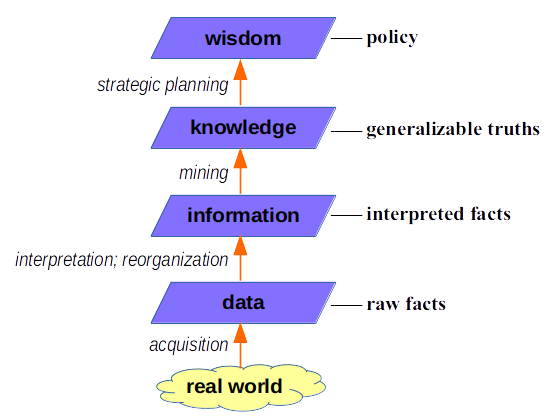
\includegraphics[width=0.9\textwidth]{dataHierarchy.png}
\caption{The data-to-wisdom hierarchy.}
\label{dataHierarchy}
\end{figure}

\subsection{The real world}
\index{real world}
\index{acquisition}

Ultimately, what we're interested in is not data, but aspects of the
\textbf{real world} -- album sales and video views, stock prices and employment
rates, hurricane trajectories and virus hot spots, or whatever. Data science
can't really get off the ground until some sort of \textbf{data acquisition}
takes place that records measurements of the real world in electronic form.

This sounds obvious, but it's important to keep in mind, actually. No matter
how much time we spend working with data, \textit{it's never the data that
actually matters -- it's the real-world phenomenon the data represents.} It
might seem strange to say that ``data'' is merely incidental to a data
scientist, but it's true. And I've definitely seen more than one data scientist
get so locked on to the data that they forget this basic truth.

One important observation is that decisions about exactly \textit{which} data
to acquire from the real world are often crucial in how things are interpreted
later on. To take an example close to home, let's say we're gathering
information on college professors so we can gauge which universities have the
highest performing faculty, and how this might be changing over the years. We
choose some representative set of criteria to measure for each faculty member
to get a rough assessment of their performance. Let's say we choose three
things: the number of research papers the professor publishes each year, the
total amount of research funding they've been granted, and the average student
evaluation score of the courses they teach. That seems like a good first cut at
assessing ``faculty performance.'' We then go on our merry data science way,
finding correlations, making data visualizations, and drawing conclusions.

This is all fine and dandy, provided we always keep in mind that it was those
three qualities, and \textit{only} those three, that we gathered in the first
place. If our study gains any traction, and university professors find they
have a vested interest in being ranked high in our yearly study, we'll discover
that they act to maximize \textit{only} the categories that are being
collected. We didn't gather data on how many university committees they served
on, or how many independent studies they supervised, or how many advisees they
had, \textit{etc.} Those metrics will inevitably become minimized in
importance, because they weren't part of what we lifted out of the real world
and onto the bottom rung of our lofty chain.

\index{GDP}
\index{Dow Jones Industrial Average}
\index{stock market}

The moral is: what we measure matters, often more than we realize. Our
country's GDP and the Dow Jones Industrial Average are easy things to quantify,
and so we often do. And thus they gain great importance in analyses of the
economy. But are they actually the most important indicators? Does focusing on
them leave out other, perhaps more vital, benchmarks? I'll just leave you with
that question for now.

\subsection{Data}

\index{gobbledy-gook}
\index{data}
\index{interpretation}

Have you ever gotten blood work done, say for an annual physical? I have. I
like to look over the numbers when the doctor hands me the results, just to
chuckle and wonder what they all mean. To me, a non-physician, they're all
pretty much gobbledy-gook. They tell me my TBC is 4.93 x10E6/$\mu$L, that
I have 5.7 Absolute Neutrophils, and a slightly out-of-range NT-proBNP (just
53.49 pg/mL, whatever the heck that means).

When I use the word \textbf{data} in the context of the hierarchy, this is what
I mean: recorded measurements, often (but not always) quantitative, that have
not yet been \textbf{interpreted}. They may be very precise, but they're also
quite meaningless without the context in which to understand them. They'd even
be meaningless to a \textit{physician} if I didn't provide the labels; try
telling your doctor that you have 4.93 ``something'' and see whether he/she
freaks out.

The good news is that when we're at the data stage of the hierarchy, we at
least have the stuff in an electronic form so we can start to \textit{do}
something with it. We also often make choices at this stage about how to
\textbf{organize} the data, choosing the appropriate type of atomic and/or
aggregate data structures that we'll discuss in detail in
Chapters~\ref{ch:atomicData} and beyond. This will allow us to bring our
analysis equipment to bear on the problem in powerful ways.

\subsection{Information}
\index{information}

Data becomes \textbf{information} when it \textit{informs} us of something;
\textit{i.e.}, when we know what it means. Getting large amounts of data
organized, formatted, and labeled the right way are jobs for the data
scientist, since turning that morass into useful knowledge is impossible
without those steps. When the aspects of the real world that we've collected
are properly structured and conceptually meaningful, we're in business.


\subsection{Knowledge}
\index{knowledge}
\index{generalizable truths}

Now \textbf{knowledge} is where the real action is. As shown in
Figure~\ref{dataHierarchy}, knowledge consists of \textit{generalizable}
truths.

\index{Chandra}
\index{Alex}
\index{bank teller}

Here's what I mean. Information is about specific individuals or occurrences.
When we say ``Chandra is a female bank teller, and earns \$48,000 a year,'' or
``Alex is a male bank teller, and earns \$69,000 a year,'' we have in our
information repository some individual facts. They can be looked up and
consulted when necessary, as you'll learn in the first part of this book.

But if we say ``women make less money than men do, even at the same jobs,''
we're in a different realm entirely. We have now generalized from specific
facts to more wide-reaching tendencies. In the language of our discipline,
we've moved from information to knowledge.

Properly gleaning knowledge from information is a trickier business than
interpreting individual data points. There are established rules, some of them
mathematical, for determining when an apparent pattern is actually reliable,
what kinds of relationships can be detected with data, whether a relationship
is causal, and so forth. We'll build some important foundations with this kind
of reasoning in this \textit{Crystal Ball} volume and its follow-on companion.
For now, I only want to make the point that \textit{knowledge} -- as opposed to
mere information -- opens up a whole new world of understanding. No longer is
the world limited to a chaotic collection of individual observations: we can
now begin to understand the general ways in which the world works...and perhaps
even to change them.

\subsection{Wisdom}
\index{wisdom}

\textbf{Wisdom} is the gold standard. It represents what we \textit{do} with
our knowledge. Let's say we indeed determine that on average men are paid
higher than women in our country, even for the same jobs. What do we do with
that realization? Is it okay? Do we want to try and fix it, and if so, how?
With laws? Education? Government subsidies? Revolution?

\index{simulation}
\index{uncertainty}

You'll remember my definition of Data Science on p.~\pageref{dsDefinition}:
deriving \textit{knowledge} from \textit{data}. This implies that the
``wisdom'' level of the hierarchy is really outside the discipline, and belongs
to other disciplines instead. And that's partially true: in some sense, the
data scientist's job stops when the deep truths about the real world are
ferreted out and illustrated, leaving it to CEOs, directors, and other policy
makers to act on them. But the data scientist is often involved here too, for a
simple reason: a decision maker wants to know what's likely to \textit{happen}
if a particular policy is implemented. Most non-trivial interventions will have
results that are hard to predict in advance, as well as unintended side
effects. One set of tools in the data scientist's toolkit is for making
principled, calculated predictions about such things, as well as quantifying
the level of \textbf{uncertainty} in the predictions. Sometimes, the technique
of \textbf{simulation} is used -- carrying out experiments on virtual societies
or systems to see the likely aggregate effects of different interventions. It's
like having a high-dimensional, multi-faceted crystal ball that lets you play
out various scenarios to their logical conclusions.

\bigskip

Starting with the rough and tumble real world and helping produce wise
decisions about how humankind can deal with it all: that's the grand promise of
the data science enterprise. And those are the mighty waters you're about to
dip your toes in! I hope you'll find it as exhilarating as I do.

% TODO: Applications (sports, Netflix, image recognition, Google, NLP,
% Coronavirus)


\section{A word of warning}

\index{Spiderman}

Before we dive into the nitty gritty, let me leave you with one more general
thought. It's actually a paraphrase of something Spiderman once said: ``with
great power comes great responsibility.''

% It's dangerous because people will believe you!

% with great power comes great responsibility
